% Section II: Background

MIMO technology is one of the most important technologies to improve the system performance in capacity, coverage and the user data rates. The performance gains depend on the propagation characteristics of each scenario. Wi-Fi, LTE, and many other radio both RF as well as wireless technologies use the new MIMO wireless technology to increase the link capacity, spectral efficiency and the link reliability using interference paths.

Rayleigh fading of signals yields a very large performance loss by converting the exponential dependency of bit error probability $P_b$ on the mean received bit energy-to-noise ratio $E_b/N_0$ into an inverse linear one. Diversity is one remedy that improves the reliability of communication by providing the receiver with multiple independently-faded copies of the same information. These copies are often referred to as diversity branches. Diversity methods can be categorized as those that exploit (1) spatial, (2) angle, (3) polarization, (4) frequency, (5) multipath, and (6) time diversity. At the receiver, the diversity branches are combined together, with the most effective combining method depending, among other things, on the type of additive impairment. For additive white Gaussian noise (AWGN) dominant channels, maximal ratio combining (MRC) is optimal in the maximum likelihood (ML) sense. For co-channel interference (CCI) dominant channels, optimum combining performs better.

The performance of a diversity scheme is measured by its diversity gain, defined as the number of independent receptions of the same signal. The independent copies of the signal increase the signal-to-interference ratio and allow a reduction in transmission power without a performance loss. A MIMO system with $N_T$ transmit antennas and $N_R$ receive antennas has a maximum diversity gain equal to $N_TN_R$.

The remainder of this section discusses the following diversity schemes, as these are the most commonly used.
\begin{itemize}
\item \emph{Time diversity}: In time diversity, a message is transmitted at different times, e.g. using different timeslots and channel coding. 
\item \emph{Frequency diversity}: In this form we use different frequencies. It may be in the form of using different channels, or technologies such as spread spectrum OFDM. 
\item \emph{Space diversity}: Space diversity is used as the basis for MIMO. It uses the antennas that are located in multiple positions to take advantage of the different radio paths that exist in a typical environment. 
\end{itemize}

\subsection{Time Diversity}
In time diversity, the fading of the channel is averaged over time by using channel coding and interleaving of code words. Thus, if a deep fade occurs, parts of many code words are affected rather than all of one code word. In this way, the error burst caused by the fade is spread out among many code words so that the error correcting code can handle the fading error.

\subsection{Frequency Diversity}
In frequency diversity, rather than spreading out signals in time, signals are spread out in frequency, which is called spread spectrum. Two common methods for spread spectrum are frequency hop spread-spectrum and direct sequence spread-spectrum.

Frequency hopping is one of two basic modulation techniques used in spread spectrum signal transmission. It is the repeated switching of frequencies during radio transmission, often to minimize the effectiveness of "electronic warfare" - that is, the unauthorized interception or jamming of telecommunications. It also is known as frequency- hopping code division multiple access (FH-CDMA).

In an FH-CDMA system, a transmitter "hops" between available frequencies according to a specified algorithm, which can be either random or preplanned. The transmitter operates in synchronization with a receiver, which remains tuned to the same center frequency as the transmitter. A short burst of data is transmitted on a narrowband. Then, the transmitter tunes to another frequency and transmits again. The receiver thus is capable of hopping its frequency over a given bandwidth several times a second, transmitting on one frequency for a certain period of time, then hopping to another frequency and transmitting again. Frequency hopping requires a much wider bandwidth than is needed to transmit the same information using only one carrier frequency.

In direct sequence spread spectrum, the stream of information to be transmitted is divided into small pieces, each of which is allocated across to a frequency channel across the spectrum. A data signal at the point of transmission is combined with a higher data-rate bit sequence (also known as a chipping code) that divides the data according to a spreading ratio. The redundant chipping code helps the signal resist interference and also enables the original data to be recovered if data bits are damaged during transmission.
In general, frequency-hopping devices use less power and are cheaper, but the performance of DS-CDMA systems is usually better and more reliable.

\subsection{Spatial (Antenna) Diversity}
In spatial diversity, many copies of the signal in uncoded transmission or coded versions of multiple signals are sent using multi-antenna systems, so each copy undergoes different fading. This diversity method is commonly referred to as MIMO. See figure~\ref{fig:mimo} for a depiction of a general MIMO system.

\begin{figure}
\centering
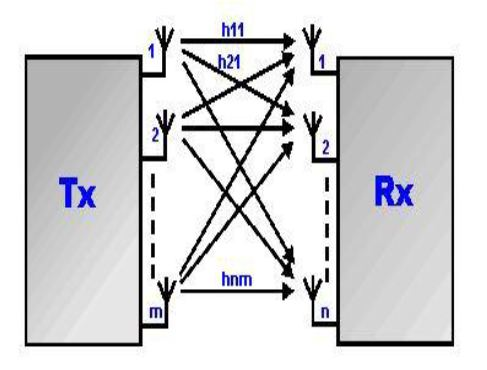
\includegraphics[width=0.6\textwidth]{images/MIMO_System.jpg}
\label{fig:mimo}
\caption{General MIMO system.}
\end{figure}

It is found that in between a transmitter and receiver, the signal can travel through multiple paths. So moving the antennas by even a small amount will lead to a change. The different number of paths that are available occurs as a result of a number of objects that appear in the direct path between the transmitter and receiver. Before these paths were just used to introduce interference but now using MIMO they can be used as an advantage. The two main formats of MIMO are: 
\begin{itemize}
\item \emph{Spatial diversity}: This refers to transmit and receive diversity. They provide improvement in the SNR and are characterized by boosting the reliability of the system with respect to fading. 
\item \emph{Spatial multiplexing}: This provides additional data capacity by using the different paths to carry traffic, thereby increasing the total throughput of the system. 
\end{itemize}
Since we use multiple antennas, MIMO can increase the capacity of a channel and still obey Shannon’s Law. With every pair of antennas that are added to the network, it is possible to linearly boost the throughput by increasing the receive and transmit antennas. Since the spectrum bandwidth is a very valuable commodity, such techniques are necessary to use the bandwidth that is available more efficiently and MIMO is one of those valuable techniques.

There are a number of MIMO configurations or formats that have been used. Each format has its own advantages and disadvantages and they can be used and balanced to provide the optimum solution for a particular application. The different MIMO formats---SISO, SIMO, MISO, MIMO all require different number of antennas and each requires different complexity. Depending on the format post processing might be required at one end or the other.

The different forms of antenna technology refer to the single or multiple inputs or outputs which are related to the radio link. In this way the input is the transmitter as it transmits into the system and the output is receiver. The different forms of single/multiple antenna links are shown in figure~\ref{fig:mimo_config}.

\begin{figure}
\centering
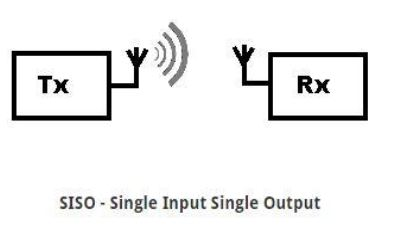
\includegraphics[width=0.4\textwidth]{images/SISO.jpg}
\qquad
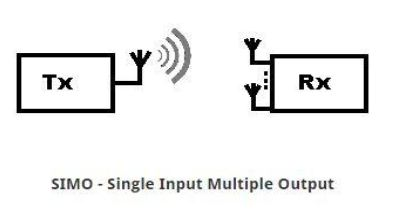
\includegraphics[width=0.4\textwidth]{images/SIMO.jpg}
\\
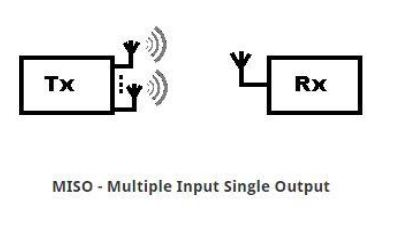
\includegraphics[width=0.4\textwidth]{images/MISO.jpg}
\qquad
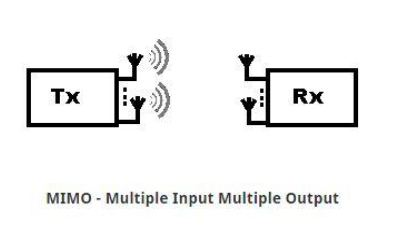
\includegraphics[width=0.4\textwidth]{images/MIMO.jpg}
\caption{Different MIMO configurations.}
\label{fig:mimo_config}
\end{figure}


\subsubsection{MIMO-SISO}
The simplest form of radio link is SISO- Single Input Single Output. In this the transmitter operates with one antenna with the receiver. In this scheme no diversity and no additional processing is required. This can be viewed from the first figure.

\subsubsection{MIMO-SIMO}
In this scheme the transmitter has a single antenna while the receiver has multiple ones. This is called as receiver diversity. This is used to support a receiver system that receives signals from a number of sources to counter the effects of fading. This scheme has been in use for a long time with short wave listening/ receiving stations to fight ionospheric fading and interference. This is represented by the second figure. The main advantage is that is easy to implement however some processing is required at the receiver side. The use of SIMO is widespread but the receiver is located as a handset, hence it may be limited by size, cost and drain.

There are two general forms of SIMO combining that can be used, namely switched diversity and maximum ratio combining. In switched diversity SIMO, the antenna switches so that it always receives the strongest signal. In maximum ratio combining, the signals from all the receive antennas are combined in proportion to the strength of the received signal.

\subsubsection{MIMO-MISO}
MISO is also called as transmit diversity, where the same data is transmitted repeatedly from two transmitters. The receiver can then extract the needed data from the optimum signal. This is represented by the third figure. The main advantage of this scheme is that the multiple antennas and the repeated coding/processing is shifted from the receiver to the transmitter. If we take the case of cellphones, this results in massive savings in terms of space and reduces the processing required for coding. Again this results in reduced batter consumption, costs and smaller size.

\subsubsection{MIMO}
In this case there are multiple antennas at the transmitter as well as the receiver. It provides advantages in total channel throughput. This scheme has been represented by the fourth and final figure. This requires coding to separate the data from the multiple paths which requires processing but boosts the total throughput and capacity.

There are many types of MIMO that can be used from SISO, through SIMO and MISO to complete MIMO networks. These are all able to provide heavy gains in performance, but usually at the expense of processing and total number of antennas. Tradeoffs have to be made between cost, performance, size, battery life before we choose the correct scheme.

%%%%%%%%

